\chapter{Introduction}
\section{Deep Learning Overview}

\subsection{Datasets}\label{sec:intro:datasets}

In this thesis manuscript, we focuses on image classification tasks and
supervised learning. Supervised learning is a machine learning paradigm in which
the model is trained using labelled data. In the context of image
classification, the input data is an image, and the label is the class of the
image. We denote an input image $X$ and its corresponding label $y$. Each image
$X$ belongs to the set of all images of the dataset $\mathcal{X}$, and each
label $y$ belongs to the set of all labels of the dataset $\mathcal{Y}$. The
dataset, denoted $\mathcal{D}$, is a set of pairs $(X, y)$, where $X \in
\mathcal{X}$ and $y \in \mathcal{Y}$, so that $D \subset \mathcal{X} \times
\mathcal{Y}$. \\

In our experiments, we evaluated our methods on three different datasets
tailored for image classification: CIFAR-10 \cite{CIFARdataset}, CIFAR-100
\cite{CIFARdataset} and TinyImageNet \cite{TinyImageNet}. The following
paragraphs give details about these datasets and \cref{tab:intro:datasets} sums
up their main characteristics.\\

\begin{table}[ht!]
    \centering
    \begin{tabular}{lcccc}
      \toprule
      \textbf{Dataset}    & \textbf{Number of images} & \textbf{Number of classes} &
      \textbf{Image size} & \textbf{Size of test set}                                               \\
      \hline
      CIFAR-10             & 60,000                    & 10                         & 32x32 & 10,000 \\
      CIFAR-100            & 60,000                    & 100                        & 32x32 & 10,000 \\
      TinyImageNet        & 100,000                   & 200                        & 64x64 & 10,000 \\
      \bottomrule
    \end{tabular}
    \caption{The number of images, of classes, image size and size of the test
    set for the three datasets used: CIFAR-10, CIFAR-100 and TinyImageNet.}
    \label{tab:intro:datasets}
  \end{table}

\noindent\textbf{CIFAR-10.} The CIFAR-10 dataset \cite{CIFARdataset} is a widely
used dataset in machine learning and computer vision. This is a labeled subset
of the \emph{80 Millions Tiny Images} dataset \cite{4531741}. CIFAR-10 is a
simple yet challenging dataset that allows for quicker iteration or
hyperparameter tuning than larger datasets such as ImageNet
\cite{DBLP:journals/ijcv/RussakovskyDSKS15}, but it is significanly more complex
than the MNIST dataset \cite{6296535}, which contains grayscale handwritten
digits images. the CIFAR-10 dataset contains 60,000 colour images of size 32x32
pixels, split into 10 classes, namely: plane, car, bird, cat, deer, dog, horse,
ship, truck. Each class contains 6,000 images. The dataset is divided into two
sets: a training set, composed of 50,000 images and a test set containing 10,000
of them.\\

\begin{figure}[ht!]
    \centering
    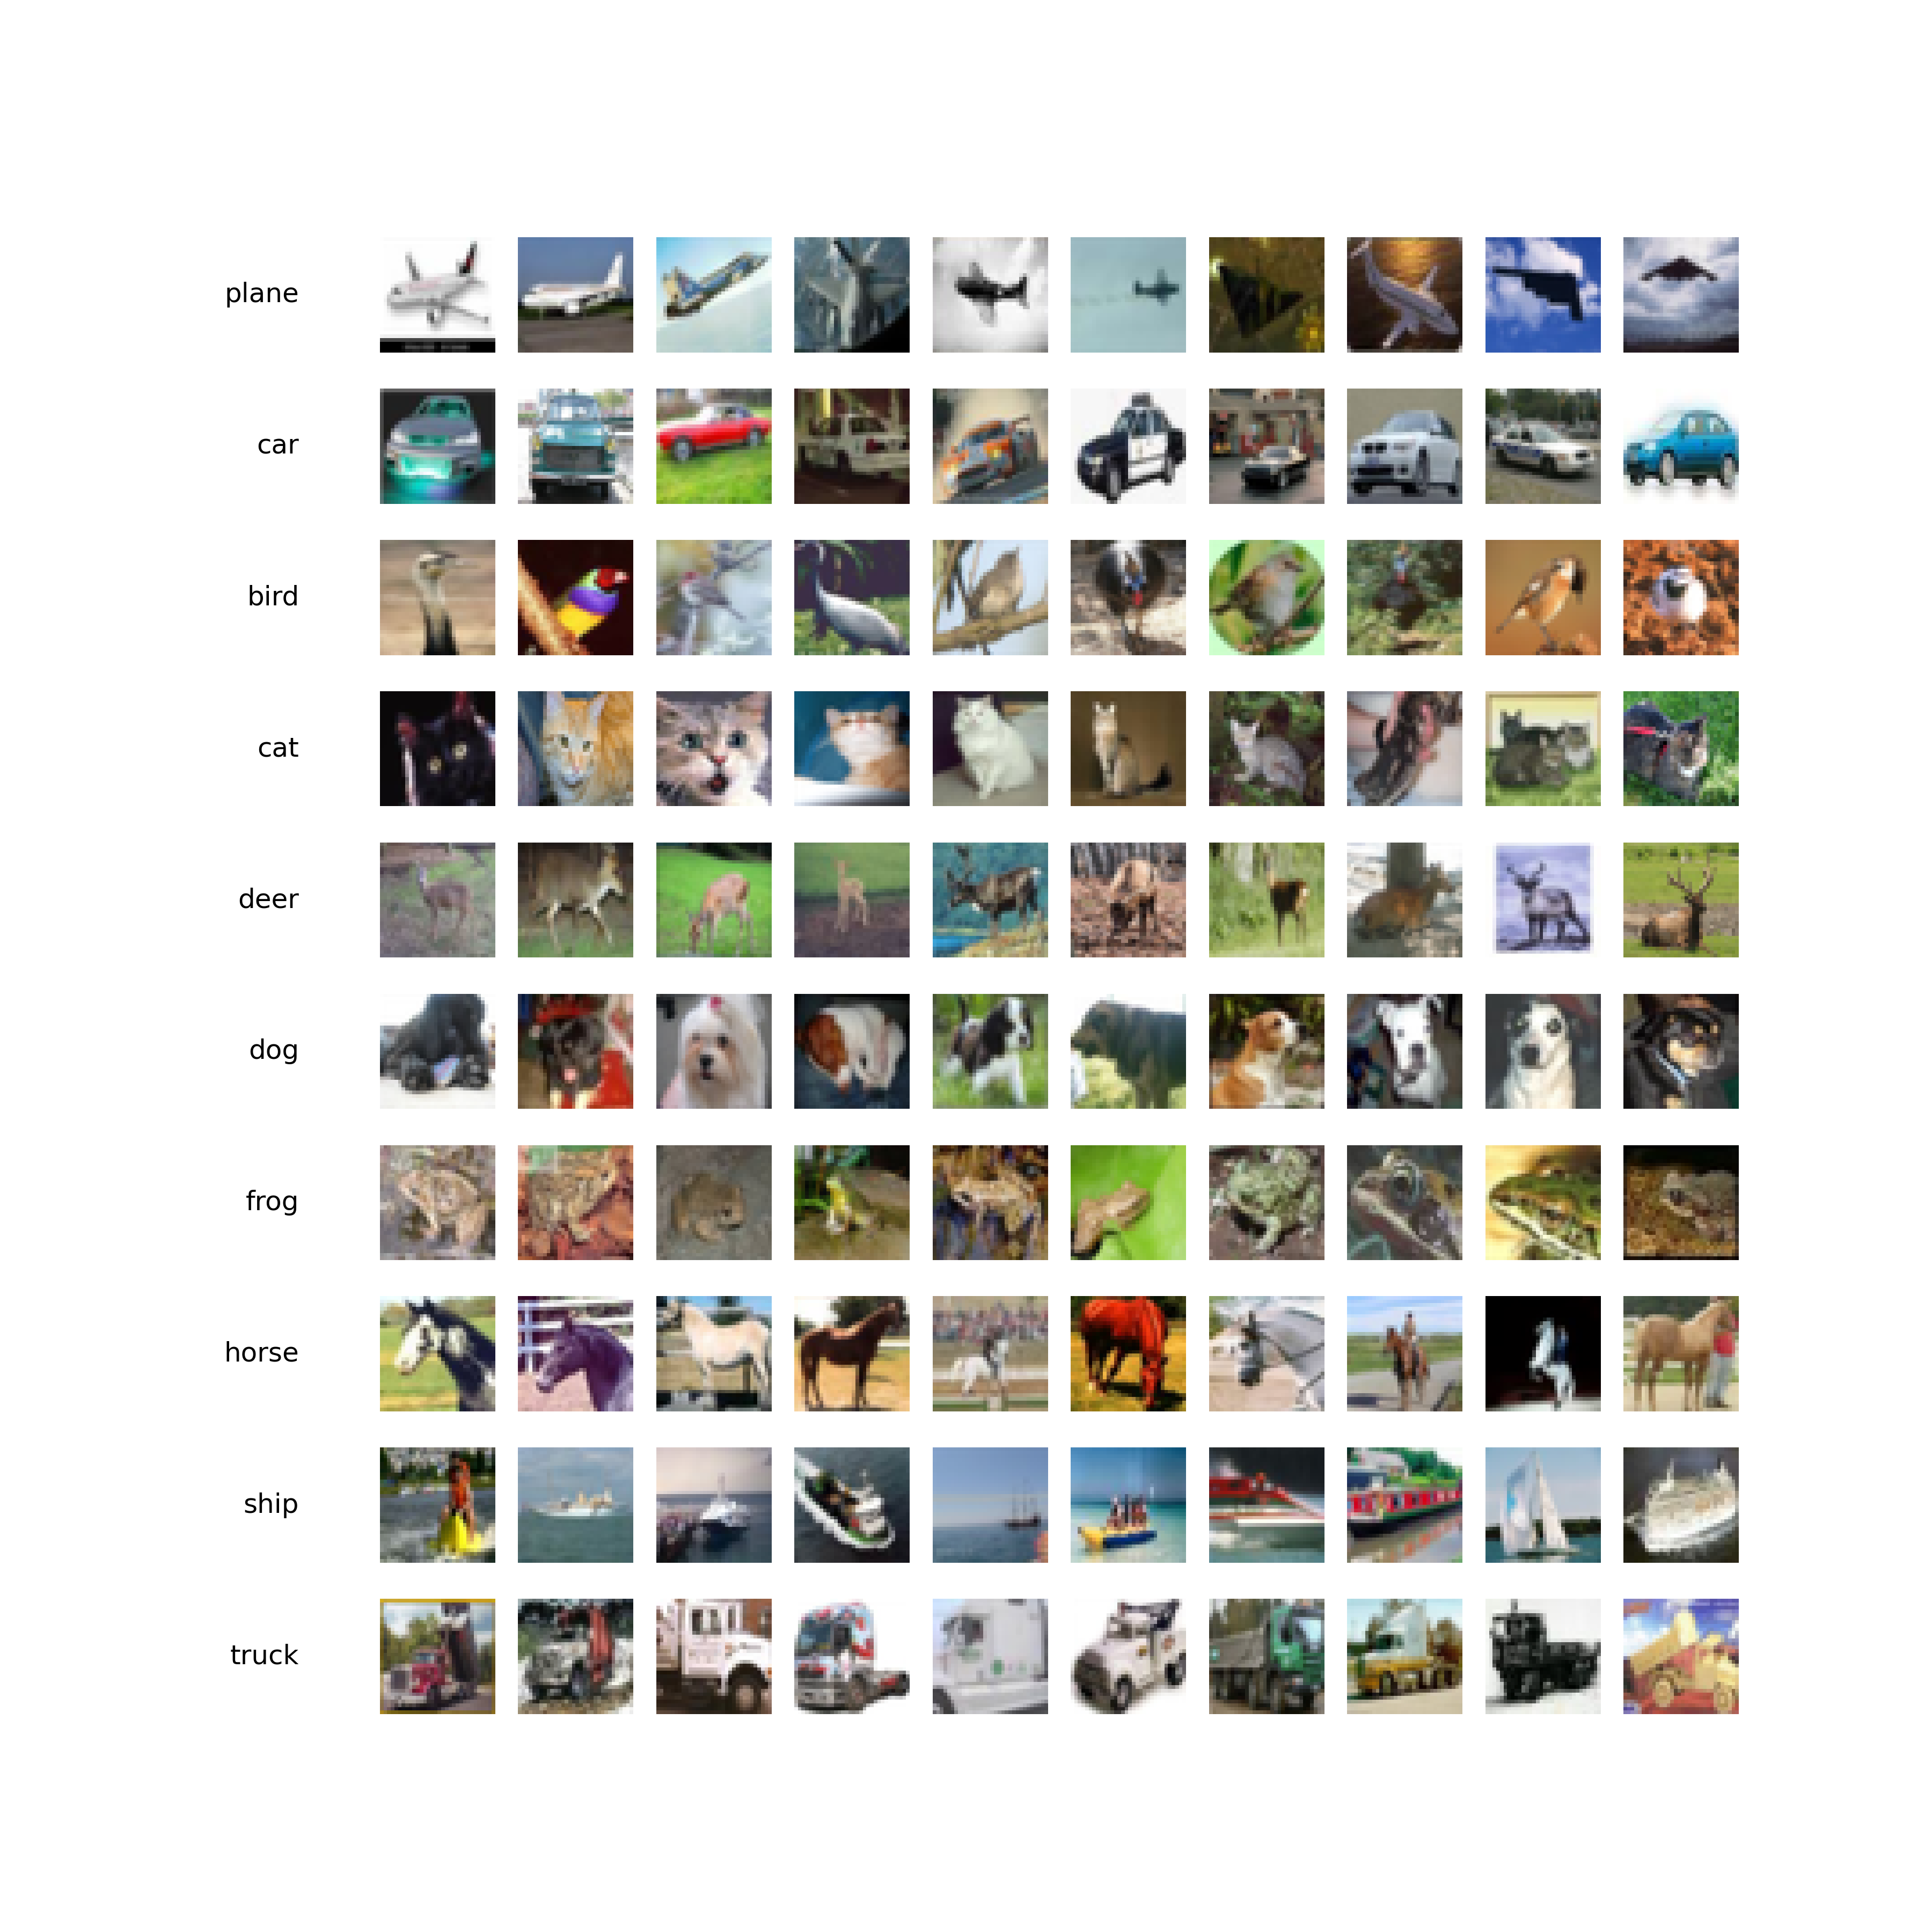
\includegraphics[width=0.7\textwidth]{chapter_intro/assets/cifar-10_example.png}
    \caption{ A sample grid of images from the CIFAR-10 dataset. Each row
    contains images from one of the 10 classes: plane, car, bird, cat,
    deer, dog, frog, horse, ship, and truck}
    \label{fig:intro:cifar10_examples}
\end{figure}


\noindent\textbf{CIFAR-100.} CIFAR-100 \cite{CIFARdataset} is a more challenging
version of CIFAR-10. Like the latter, it is a labeled subset of the \emph{80
Millions Tiny Images} and  is composed of 60,000 colour images of size 32x32
pixels. However, instead of 10 classes, CIFAR-100 contains 100 classes of 600
images each. As a result, each class has far fewer images than in CIFAR-10.
CIFAR-100 is also divided into two sets: a training set and a test, composed of
50,000 and 10,000 images respectively.\\

\begin{figure}[ht!]
    \centering
    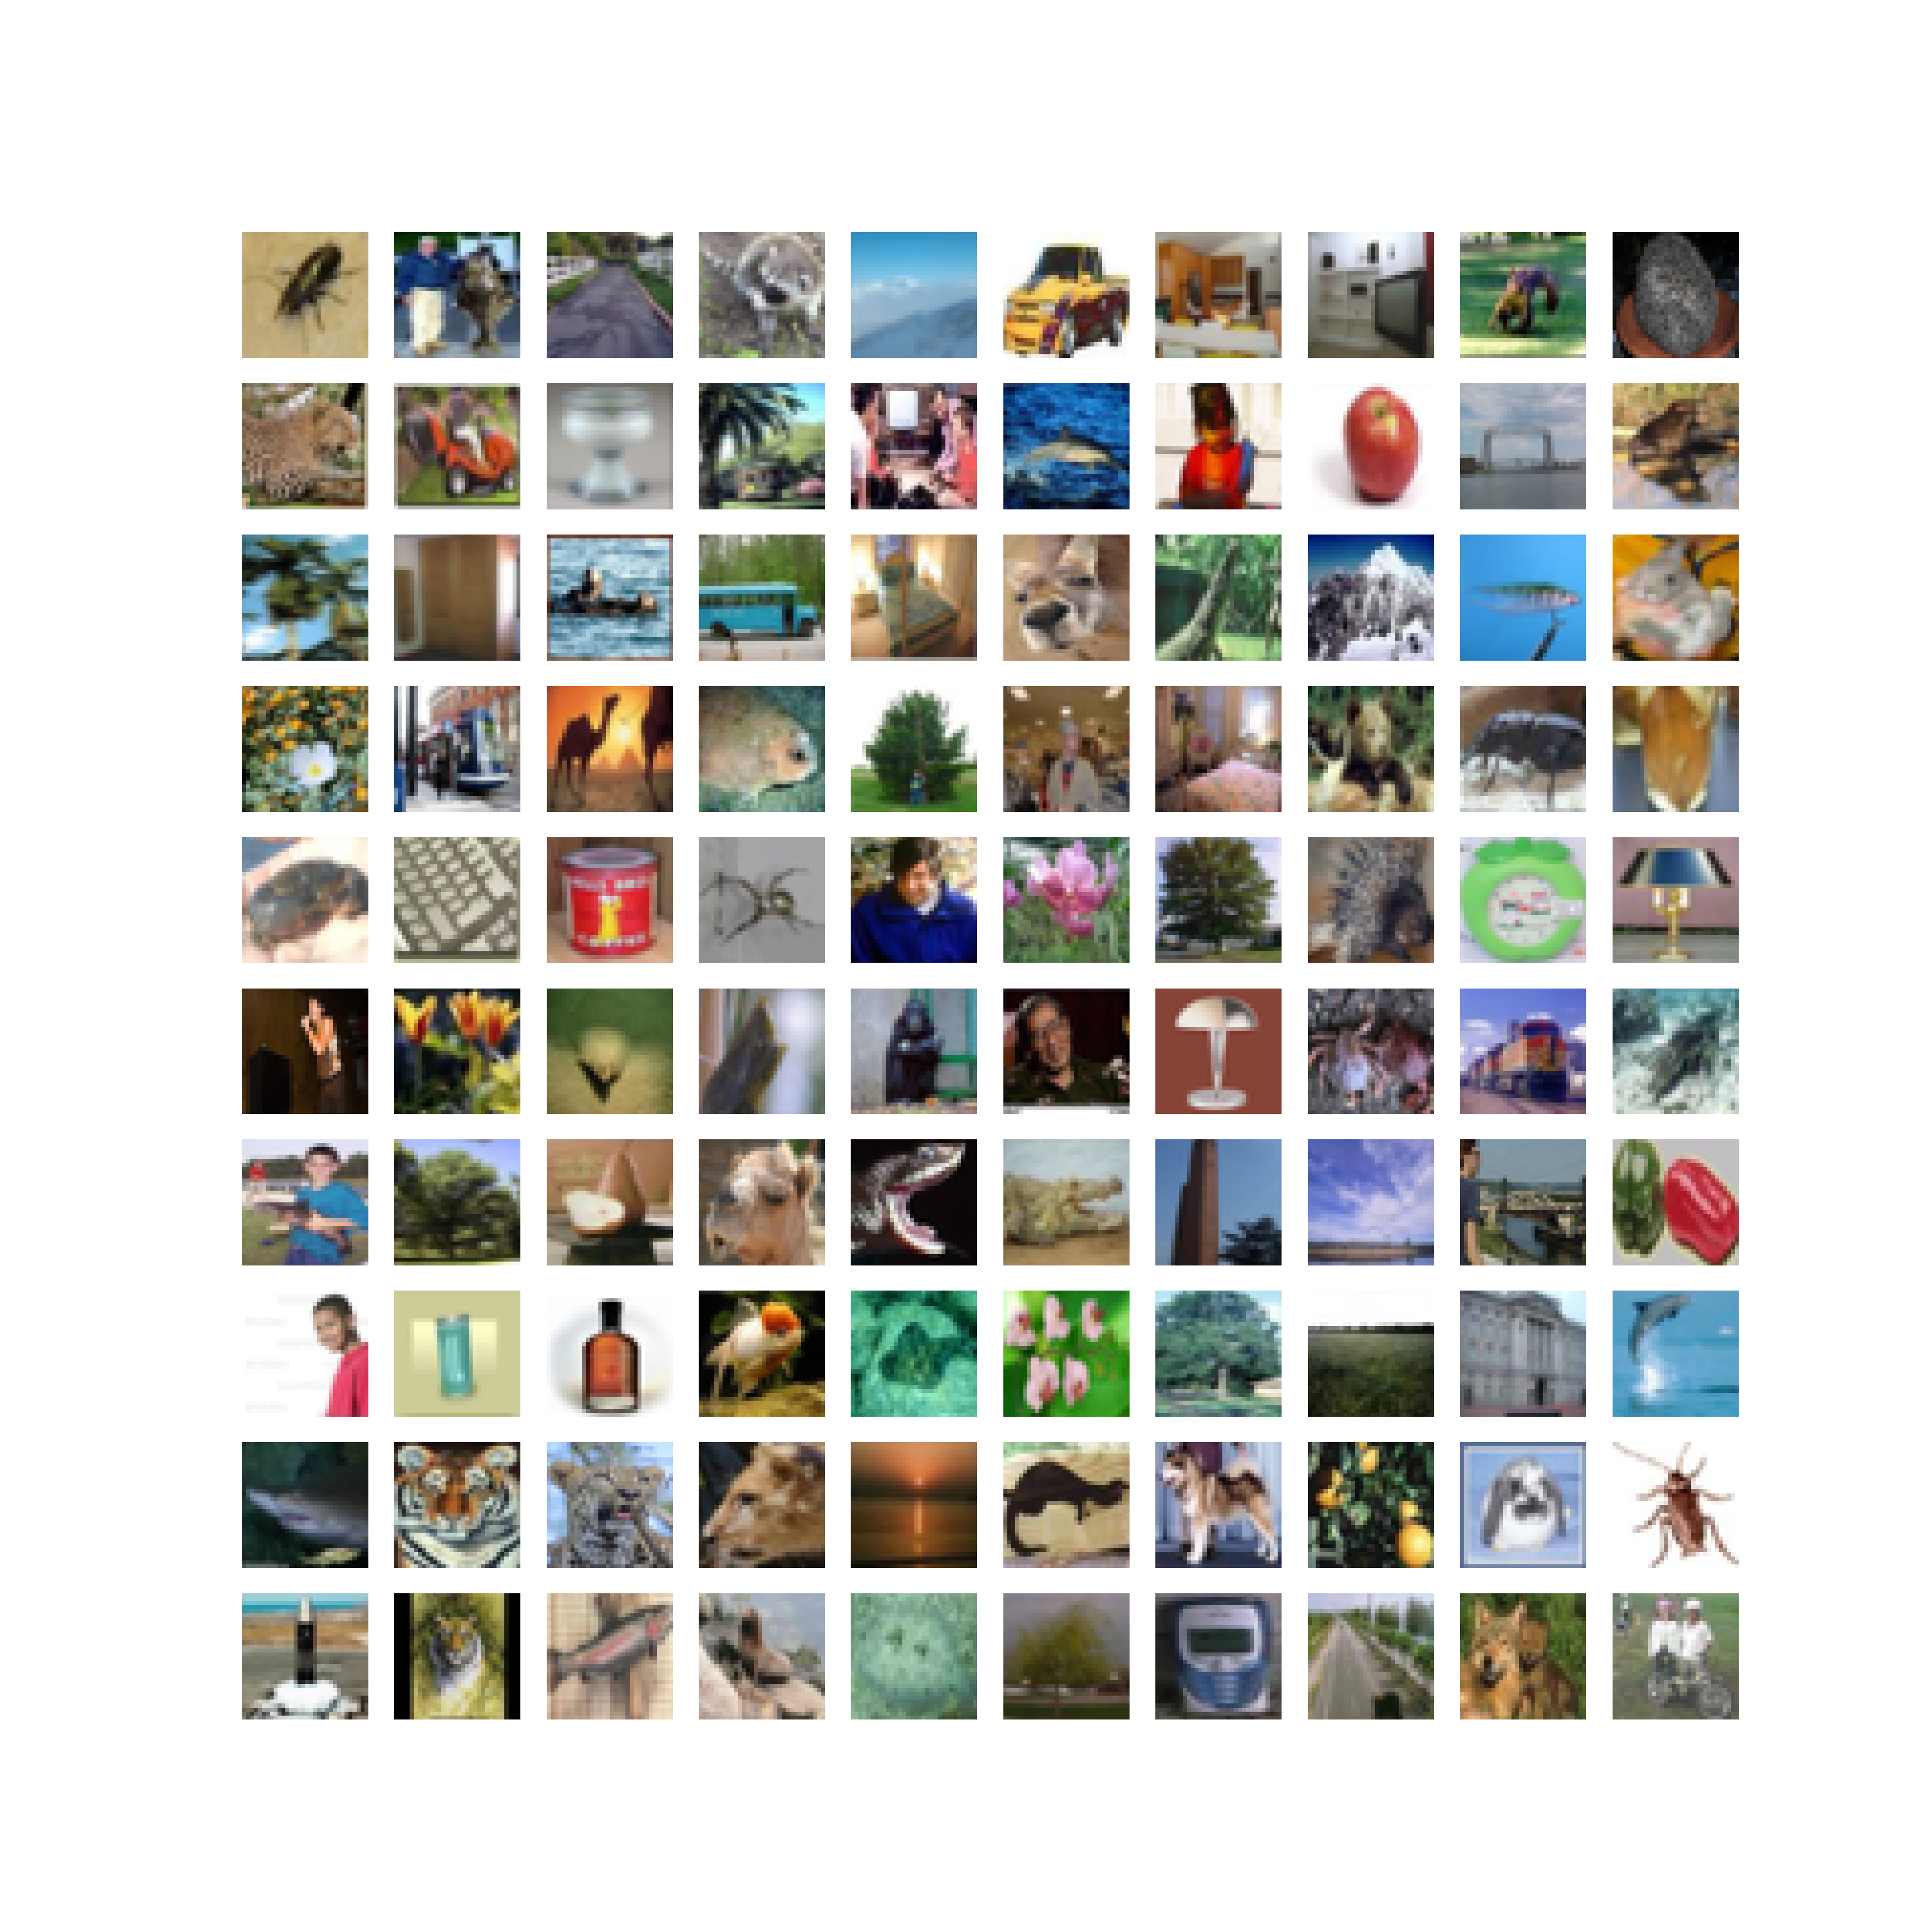
\includegraphics[width=0.7\textwidth]{chapter_intro/assets/cifar-100_example.png}
    \caption{A sample grid of images from the CIFAR-100 dataset. The images
    represent a subset of the 100 available classes, each image represents
    a unique class.}
    \label{fig:intro:cifar100_examples}
\end{figure}

\noindent\textbf{TinyImageNet.} TinyImageNet dataset is another popular dataset
in machine learning and computer vision, conceived as a subset of the larger
ImageNet dataset \cite{DBLP:journals/ijcv/RussakovskyDSKS15}. It comprises
100,000 colour images of size 64x64 pixels, split into 200 classes, whereas
ImageNet contains 1.2 million images of size 256x256 pixels, split into 1,000
classes. The dataset is divided in 3 sets: the train set, containing 500
images per class, the validation and test sets, both containing 50. The scaled
down image size and count make TinyImageNet more computationally accessible than
ImageNet while still being a challenging task and maintening the diversity of
the images and classes.\\


\begin{figure}[ht!]
    \centering
    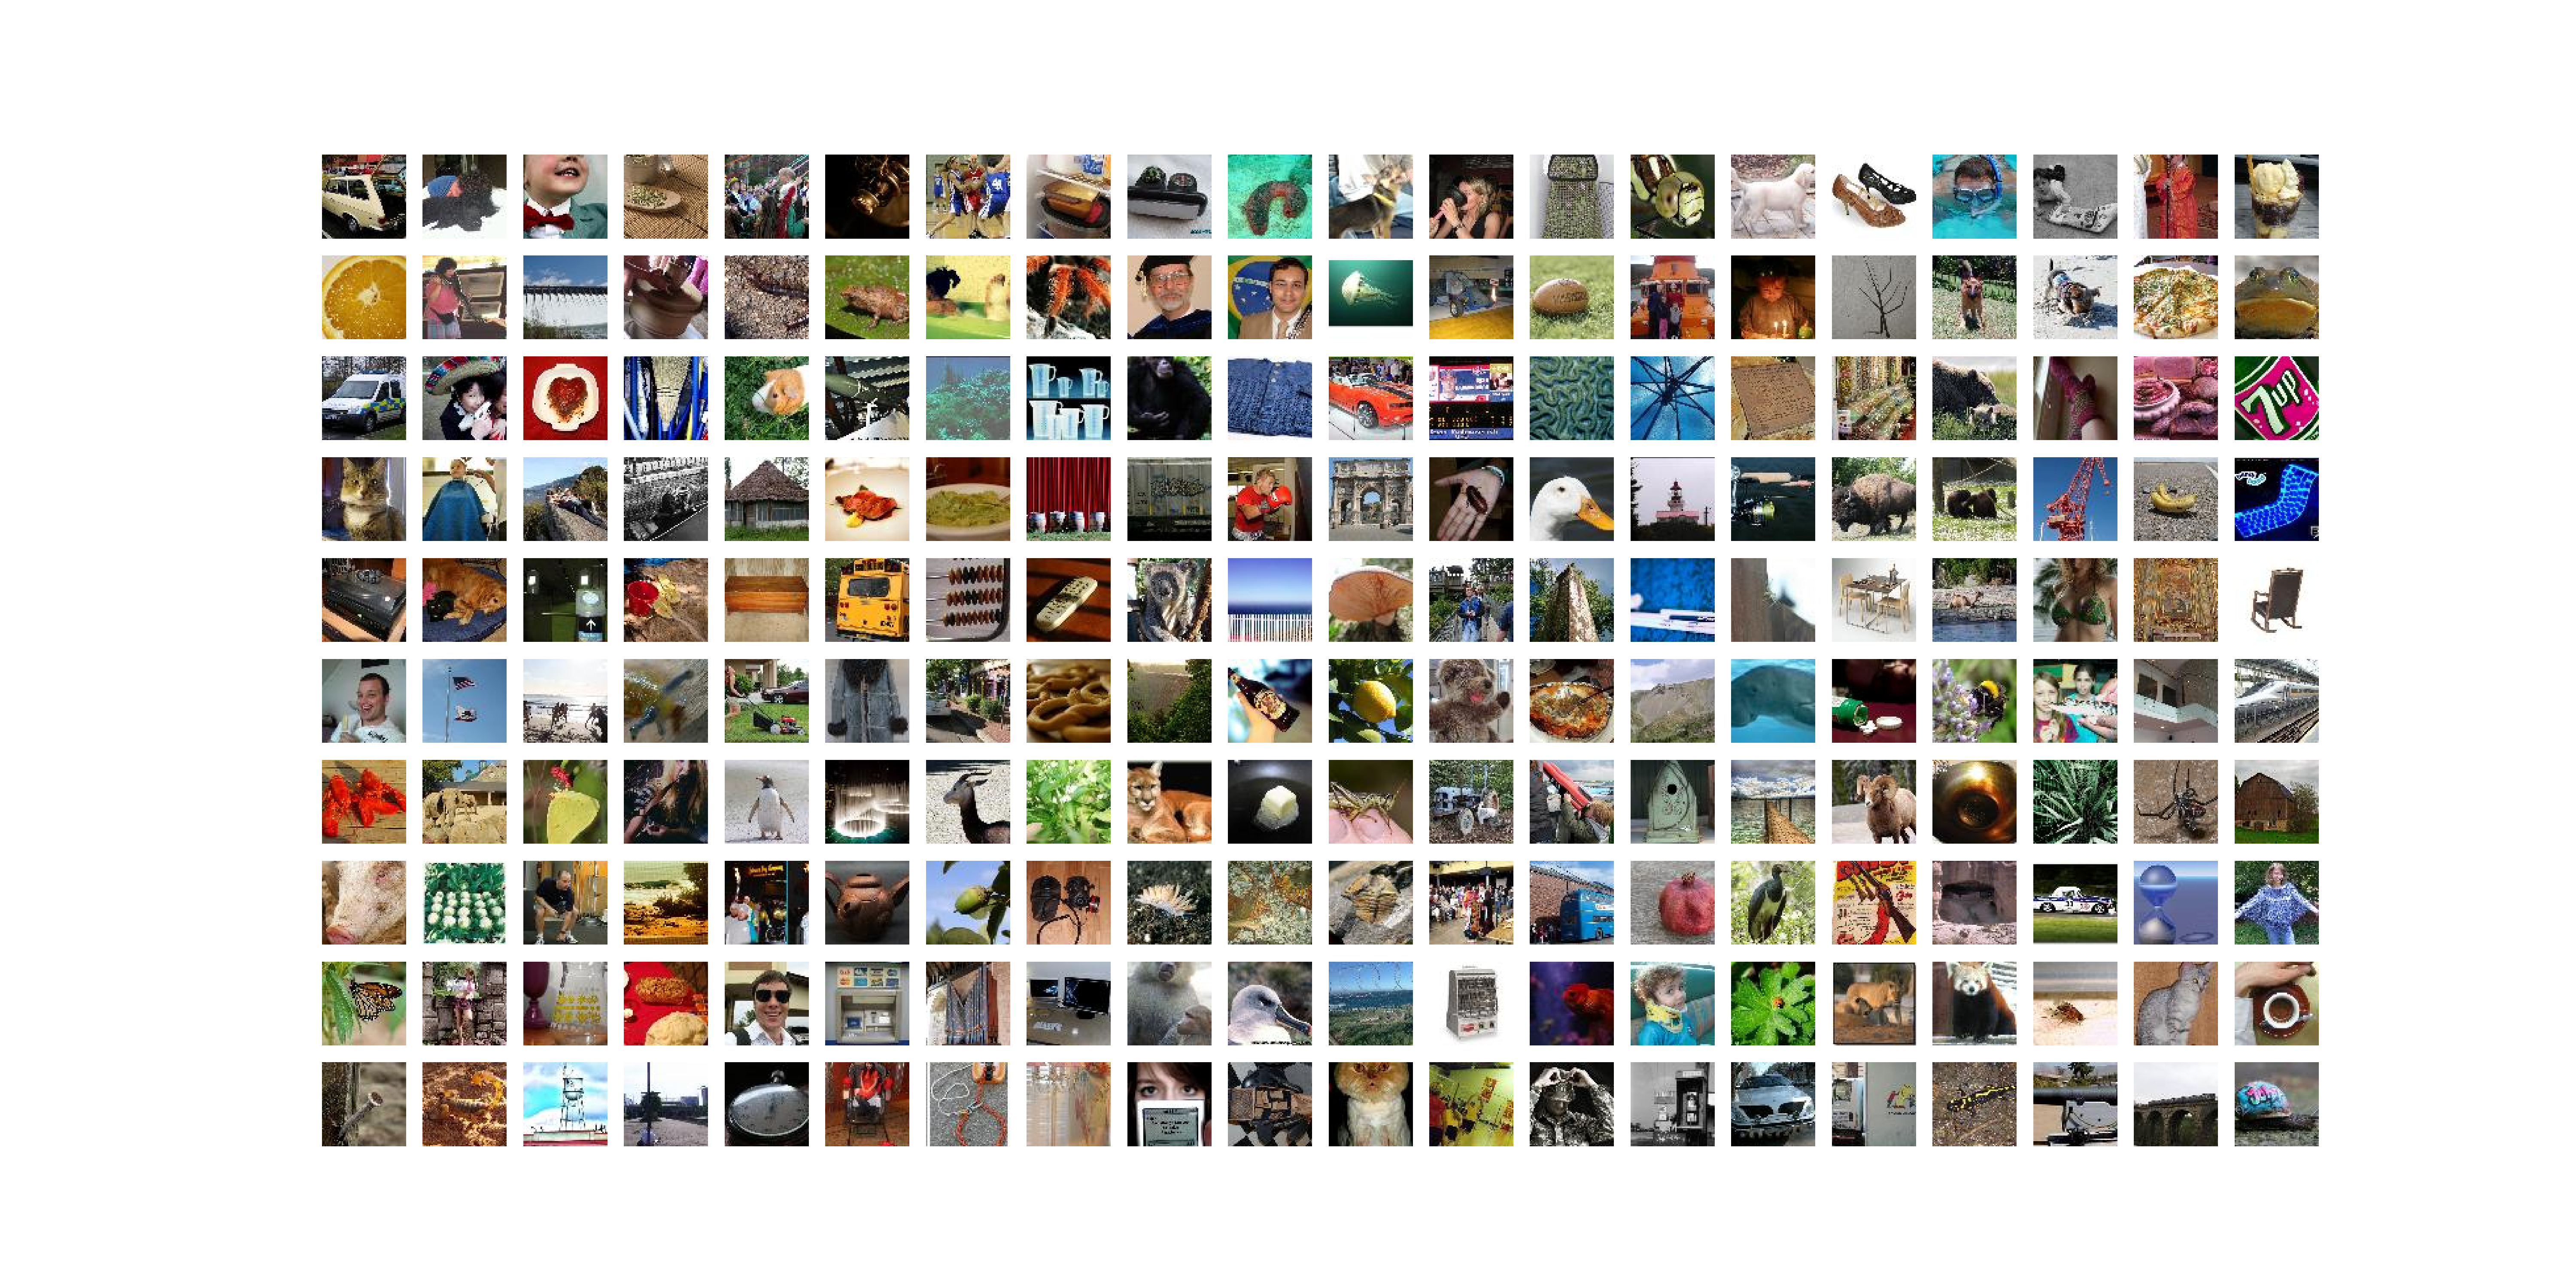
\includegraphics[width=0.7\textwidth]{chapter_intro/assets/tinyimagenet_example.png}
    \caption{A sample grid of images from the Tiny ImageNet dataset. The images
    represent a subset of the 200 distinct classes, each image represents a
    unique class.}
    \label{fig:intro:tinyimagenet_examples}
\end{figure}

% In addition to these two folds, we
% also use a validation set to tune the hyperparameters of our method before
% applying it on the test set. The validation dataset is obtained by selecting
% 10\% of the training set. \Cref{tab:intro:datasets} summaries the composition of
% the three datasets.\\ 

% The CIFAR-10 and CIFAR-100 datasets both contain 60 000 colour images of size
% 32x32 pixels, split into 10 and 100 classes, respectively. The TinyImageNet
% dataset is a shrunk version of the ImageNet dataset
% \cite{DBLP:journals/ijcv/RussakovskyDSKS15}, and contains 100 000 images of size
% 64x64 pixels, split into 200 classes. Each dataset is divided into two folds: a
% training set and a test set. In addition to these two folds, we also use a
% validation set to tune the hyperparameters of our method before applying it on
% the test set. The validation dataset is obtained by selecting 10\% of the
% training set. \Cref{tab:intro:datasets} summaries the composition of the three
% datasets.\\

% In combination with these datasets, we use four different neural networks. Conv4
% is a reasonably small convolutional neural network which is a
% shrunk-down version of the VGG16 architecture. VGG16 is a \acl{CNN}
% of larger size and depth, which is a popular choice for image classification. We
% used a slightly modified version of VGG16 that is better suited to CIFAR-10. We
% do not use dropout, but we use batch normalisation, and the fully connected
% section has only one layer. ResNet18 is a residual neural network that
% introduces skip connections in its architectural design. ResNet20 is a modified
% version of the ResNet18 architecture to make it suited for CIFAR-10 and CIFAR-100
% datasets. \Cref{tab:intro:networks_size} summarises the size of the different
% models. In our experiments, we use ResNet18 exclusively for TinyImageNet and the
% other networks for CIFAR-10 and CIFAR-100.\\

\textbf{Train, Validation and Test Sets.} 
In our experiments, for each dataset, we use 3 sets: train, validation and test
sets. The training set serves to train the model, while the validation set is
used to monitor the evolution of performance metrics on unseen data throughout
the training. Validation metrics provides the necessary triggers for the early
stopping policy (\emph{i.e.} interrupting the training prematurely if me
validation metrics do not change over a given number of iterations). The test
set, on the other hand, is used to evaluate the model's performance on entirely
new data and reporting the final test accuracy. When utilizing datasets like
CIFAR-10 and CIFAR-100, only training and testing sets are available. For these
datasets, we split the given train set in half with the following proportions:
90\% of the original training set is used for training for the network and the
remaining 10\% is used as the validation set. On the other hand, the
TinyImageNet dataset does provide training, validation, and testing sets, but
the test set lacks annotations. Hence, we use 90\% of the training set for model
training and the remaining 10\% for validation. Instead of the unannotated test
set, we repurpose the original validation set to serve as the test set. This is
a common strategy employed by other implementations
\cite{hanyuanxu2018tinyimagenet,nbdt,alvinwan2020nbdt}.\\

\subsection{Architectures}\label{sec:intro:architectures}

% Tiré du chapitre 2
Conv2 and Conv6 are modified versions of the Conv4 architecture, featuring 2 and
6 convolutional layers, respectively, instead of the original 4 convolutional
layers. The other networks mentioned are described in
\cref{sec:chap1:experiments}. The number of parameters for these architectures
is provided in \cref{tab:chap2:conv_num_params}. Although the Conv2, Conv4 and
Conv6 networks introduced by \citeauthor{DBLP:conf/iclr/FrankleC19} in
\cite{DBLP:conf/iclr/FrankleC19} are not widely featured in existing literature,
we chose to employ them due to their use in the methods we benchmark against.

\begin{table}[ht!]
    \centering\begin{tabular}{lccc}
      \cmidrule[\heavyrulewidth]{2-4}
                           & \textbf{Conv2} & \textbf{Conv4} & \textbf{Conv6} \\ \toprule
      Number of Parameters & 4,301,642      & 2,425,930      & 2,262,602      \\ \bottomrule
    \end{tabular}
    \caption{Number of parameters for the Conv2, Conv4 and Conv6 architectures, when used with the CIFAR-10 dataset}
    \label{tab:chap2:conv_num_params}
\end{table}

\begin{table}[ht!]
    \centering
    \begin{tabular}{lcccc}
      \cline{2-5}
                           & \textbf{Conv4} & \textbf{VGG16} & \textbf{ResNet20} & \textbf{ResNet18} \\ \hline
      Number of Parameters & 2,425,930      & 14,728,266     & 269,034           & 11,685,608        \\ \hline
    \end{tabular}
    \caption{ number of parameters for the four used neural network architectures.}
    \label{tab:intro:networks_size}
\end{table}